\section{Results}

To test the clustering algorithm, a terrain is loaded, it's resources edited and five clusters produced. These clusters are subsequently analysed to ensure they successfully detect distinct resource features on which to cluster.\\

The terrain used is a model of the Grand Canyon using data from the US Geological Survey \protect\footnotemark \footnotetext{\url{http://www.usgs.gov}}. This terrain is chosen as its canyons and crevasses make ground illumination vary greatly.\\

The following resource edits were performed on the terrain:

\begin{itemize}
\item \textit{Latitude}: Set to zero degrees (equator)
\item \textit{Soil Infiltration}: 5 millimetres for all terrain points with a slope under 30 degrees. All points with a slope over 30 degrees were set to 0 to simulate a cliff.
\item \textit{Rainfall}: 25 millimetres for every month.
\item \textit{Temperature}: 15 degrees at 0 meters in December. 30 degrees at 0 metres in June. 
\end{itemize}

The resulting terrain clusters that form are displayed in figure \ref{fig:clustering_test_resulting_clusters} and summarized in table \ref{tab:clustering_test_resulting_clusters}.

\begin{figure}
\center
	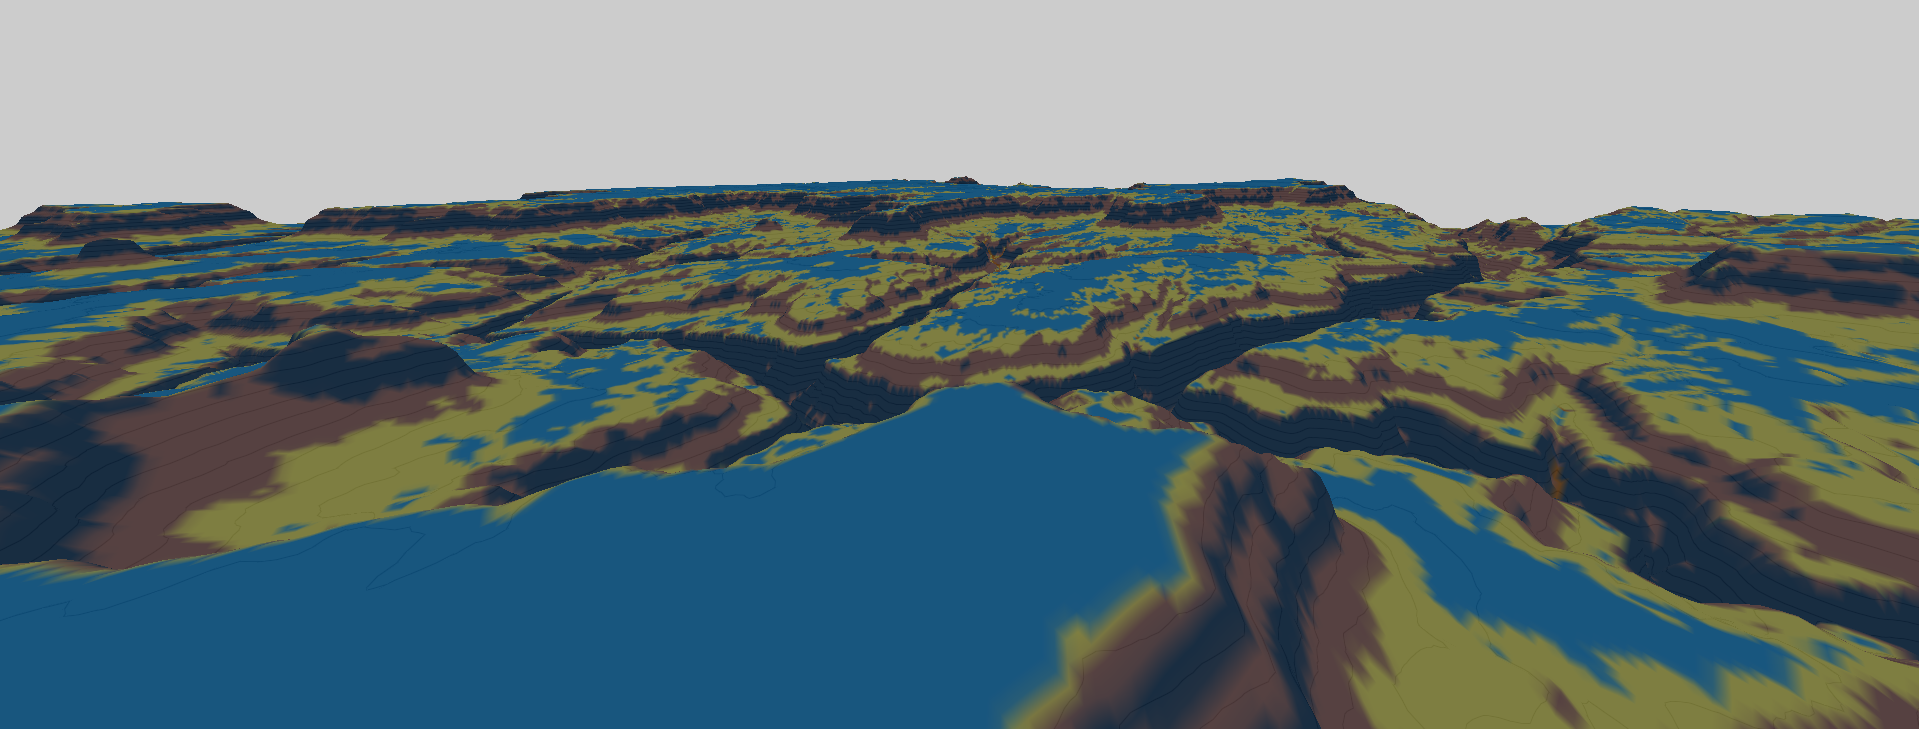
\includegraphics[width=\textwidth]{clustering_test_resulting_clusters.png}
	\caption{ Clustering test: Resulting terrain clusters}	
	\label{fig:clustering_test_resulting_clusters}
\end{figure}

\definecolor{cluster_1}{rgb}{0.8,0.4,0.0}
\definecolor{cluster_2}{rgb}{0.6,0.4,0.4}
\definecolor{cluster_3}{rgb}{0.0,0.2,0.4}
\definecolor{cluster_4}{rgb}{1.0,1.0,0.4}
\definecolor{cluster_5}{rgb}{0.0,0.6,1.0}

\begin{table}[]
  \centering
	    \begin{tabular}{|p{5cm}|p{2cm}|p{2cm}|p{2cm}|p{2cm}|p{2cm}|}
		\hline	
  	     & \textbf{1} &  \textbf{2} & \textbf{3} & \textbf{4} & \textbf{5} \\
		\hline
  	    Color & \cellcolor{cluster_1} & \cellcolor{cluster_2} & \cellcolor{cluster_3} & \cellcolor{cluster_4} & \cellcolor{cluster_5} \\
		\hline
  	    Member count & 314415 (30\%)  & 225868 (22\%) & 225943 (22\%)  & 9201 (0.8\%) & 273149 (26\%) \\
		\hline
  	    Slope & 6.65549 & 15.5914 & 16.2722 & 19.8204 & 46.483 \\
		\hline
  	    Temp (Jan) & 19 & 23 & 21 & 25 & 23 \\
		\hline
  	    Temp (Feb) & 17 & 21 & 19 & 23 & 21 \\
		\hline
  	    Temp (Mar) & 14 & 18 & 16 & 20 & 18 \\
		\hline
  	    Temp (Apr) & 12 & 16 & 14 & 18 & 16 \\
		\hline
  	    Temp (May) & 9 & 13 & 11 & 15 & 13 \\
		\hline
		Temp (Jun) & 7 & 11 & 9 & 13 & 11 \\
		\hline
		Temp (Jul) & 9 & 13 & 11 & 15 & 13 \\
		\hline
		Temp (Aug) & 12 & 16 & 14 & 18 & 16 \\
		\hline
		Temp (Sep) & 14 & 18 & 16 & 20 & 18 \\
		\hline
		Temp (Oct) & 17 & 21 & 19 & 23 & 21 \\
		\hline
		Temp (Nov) & 19 & 23 & 21 & 25 & 23 \\
		\hline
		Temp (Dec) & 22 & 26 & 24 & 28 & 26 \\
		\hline
  	    Illumination (Jan) & 8 & 5 & 6 & 3 & 4 \\
		\hline
  	    Illumination (Feb) & 9 & 6 & 7 & 4 & 4 \\
		\hline
  	    Illumination (Mar) & 9 & 7 & 8 & 5 & 5 \\
		\hline
  	    Illumination (Apr) & 10 & 8 & 9 & 6 & 6 \\
		\hline
  	    Illumination (May) & 11 & 9 & 10 & 6 & 7 \\
		\hline
		Illumination (Jun) & 12 & 9 & 10 & 7 & 7 \\
		\hline
		Illumination (Jul) & 11 & 9 & 10 & 6 & 7 \\
		\hline
		Illumination (Aug) & 10 & 8 & 9 & 6 & 6 \\
		\hline
		Illumination (Sep) & 9 & 7 & 8 & 5 & 5 \\
		\hline
		Illumination (Oct) & 9 & 6 & 7 & 4 & 4 \\
		\hline
		Illumination (Nov) & 8 & 5 & 6 & 3 & 4 \\
		\hline
		Illumination (Dec) & 6 & 4 & 5 & 2 & 3 \\
		\hline
  	    Soil Humidity (Jan) & 24.7 & 26.8 & 23.2 & 711.4 & 2.2 \\
		\hline
  	    Soil Humidity (Feb) & 24.7 & 26.8 & 23.2 & 711.4 & 2.2 \\
		\hline
  	    Soil Humidity (Mar) & 24.7 & 26.8 & 23.2 & 711.4 & 2.2 \\
		\hline
  	    Soil Humidity (Apr) & 24.7 & 26.8 & 23.2 & 711.4 & 2.2 \\
		\hline
  	    Soil Humidity (May) & 24.7 & 26.8 & 23.2 & 711.4 & 2.2 \\
		\hline
  	    Soil Humidity (Jun) & 24.7 & 26.8 & 23.2 & 711.4 & 2.2 \\
		\hline
  	    Soil Humidity (Jul) & 24.7 & 26.8 & 23.2 & 711.4 & 2.2 \\
		\hline
  	    Soil Humidity (Aug) & 24.7 & 26.8 & 23.2 & 711.4 & 2.2 \\
		\hline
  	    Soil Humidity (Sep) & 24.7 & 26.8 & 23.2 & 711.4 & 2.2 \\
		\hline
  	    Soil Humidity (Oct) & 24.7 & 26.8 & 23.2 & 711.4 & 2.2 \\
		\hline
  	    Soil Humidity (Nov) & 24.7 & 26.8 & 23.2 & 711.4 & 2.2 \\
		\hline
  	    Soil Humidity (Dec) & 24.7 & 26.8 & 23.2 & 711.4 & 2.2 \\
		\hline
		\end{tabular}
		\caption{Clustering test: Cluster summary.}
	  \label{tab:clustering_test_resulting_clusters}
\end{table}

\begin{figure}
\center
	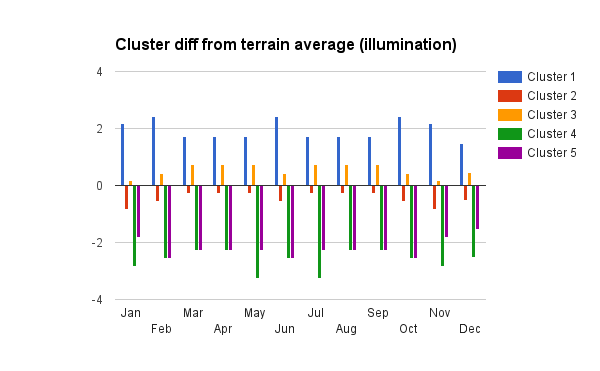
\includegraphics[width=\textwidth]{clustering_graph_illumination_diff.png}
	\caption{ Monthly illumination for each cluster and the average over the whole terrain.}	
	\label{fig:clustering_graph_illumination}
\end{figure}

\begin{figure}
\center
	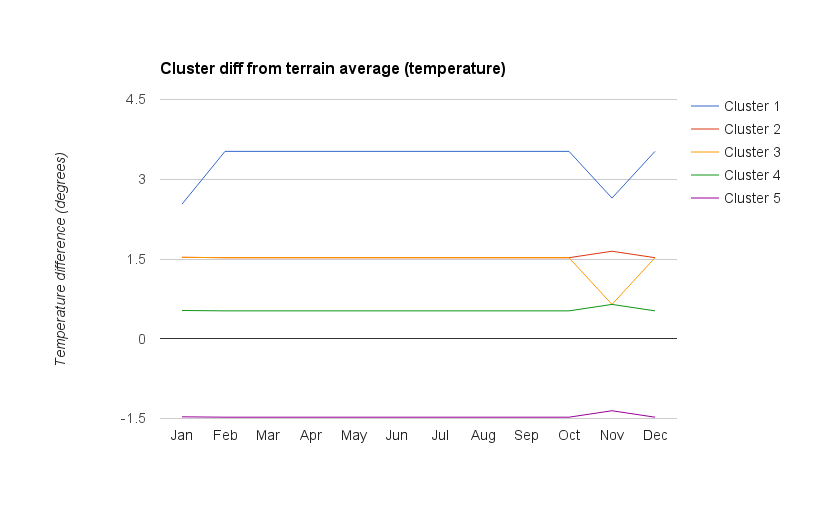
\includegraphics[width=\textwidth]{clustering_graph_temp_diff.png}
	\caption{ Monthly temperature for each cluster and the average over the whole terrain. Cluster 2 has the same values as cluster 4.}	
	\label{fig:clustering_graph_temp}
\end{figure}

\begin{figure}
\center
	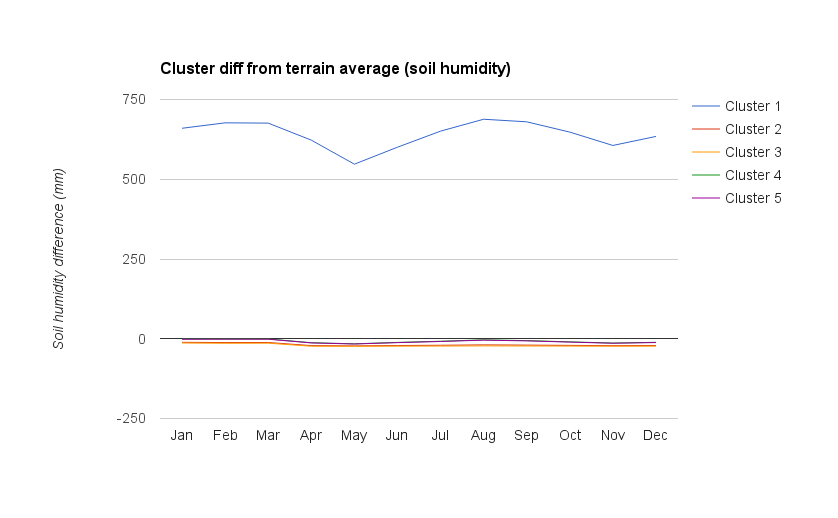
\includegraphics[width=\textwidth]{clustering_graph_soil_humidity_diff.png}
	\caption{ Soil humidity for each cluster (same for every month) and the average over the whole terrain.}	
	\label{fig:clustering_graph_humidity}
\end{figure}

\begin{figure}
\center
	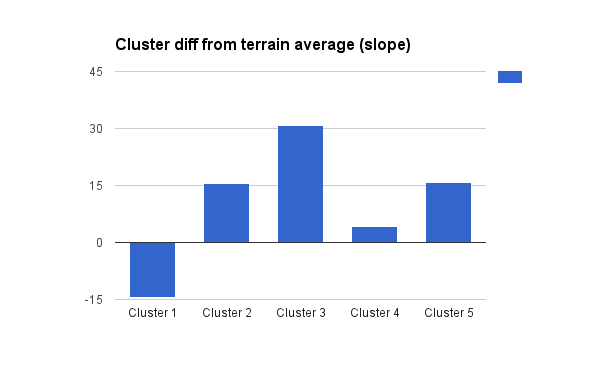
\includegraphics[width=\textwidth]{clustering_graph_slope_diff.png}
	\caption{ Slope for each cluster and the average over the whole terrain.}	
	\label{fig:clustering_graph_slope}
\end{figure}

Figures \ref{fig:clustering_graph_illumination}, \ref{fig:clustering_graph_temp}, \ref{fig:clustering_graph_humidity} and \ref{fig:clustering_graph_slope} show the cluster values along with the terrain average for illumination, temperature, soil humidity and slope respectively. Using these figures, it is possible to analytically determine the principle cluster feature(s) (see table{\ref{tab:clustering_test_cluster_analysis}). 

\begin{table}[]
  \centering
	    \begin{tabular}{|p{3cm}|p{3cm}|p{3cm}|p{3cm}|p{3cm}|}
		\hline	
  	    Cluster & Illumination &  Temperature & Soil Humidity & Slope \\
		\hline	
		1 & High & Low & Avg & Very Low\\
		\hline
		2 & Avg & High & Avg & Avg \\
		\hline
		3 & Avg & Avg & Avg & Avg \\
		\hline	
		4 & Low & High & Very High & Avg \\
		\hline	
		5 & Low & Avg & Very High & Avg \\
		\hline	
		\end{tabular}
		\caption{Cluster comparison analysis}
	  \label{tab:clustering_test_cluster_analysis}
\end{table}

